\chapter{Случайные блуждания}

\section{Понятие случайного процесса}
\begin{df}
	Пусть $(V, \Ac)$, $(S, \Bc)$ --- измеримые пространства, $f \cln V \to S$.

	$f \in \Ac \divs \Bc$ --- \textit{$(\Ac, \Bc)$--измеримое отображение}, если
	%FIXME: вместо = должно быть :=
	$\fA B \in \Bc f^{-1}(B) = \hc{x \in V | f(x) \in B} \in \Ac$

	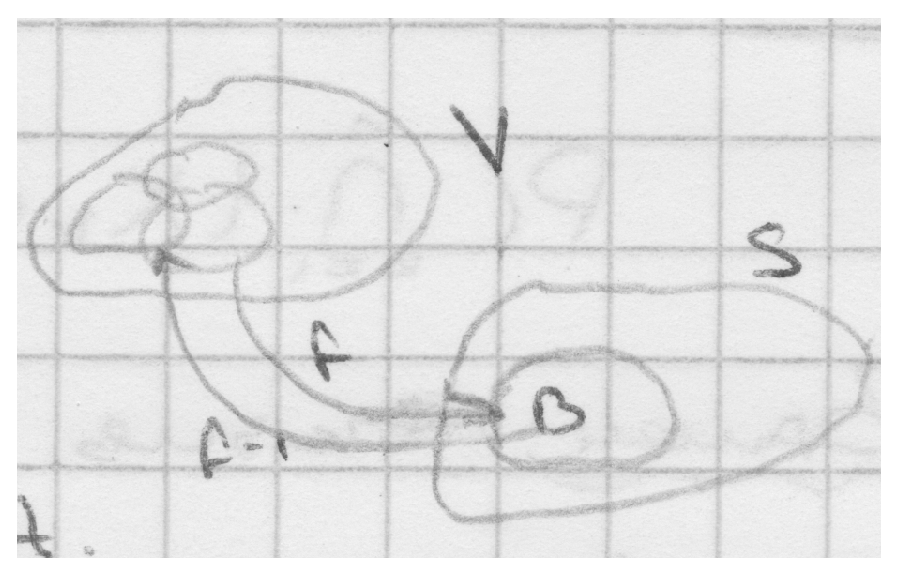
\includegraphics[scale = .3]{p0-01.eps}

	Пусть $(\Om, \Fc)$ --- измеримое.
	И пусть на нём имеется мера $\Pbb$ \sth $\Pbb(\Om) = 1$.
	Тогда $(\Om, \Fc, \Pbb)$ -- \textit{вероятностное пространство}.

	$Y \cln \Om \to S$ --- случайный элемент, если $Y \in \Fc \divs \Bc$.
\end{df}
\begin{ex}
	$S = \R^m$, $\Bc = \Bc(\R)$ --- борелевские множества.
	Тогда при $m > 1$ случайный элемент $Y$ --- случайный вектор;
	если $m = 1$, то $Y$ --- случайная величина.
	$\Pb_Y(B) = \Pb[Y^{-1}(B)]$ --- мера на $\Bc$.

	Легко видеть, что
	$$
		\Pb_Y(B) = \Pb\hc{\om \in \Om | Y(\om) \in B}
	$$
\end{ex}
